\chapter{总体设计}
\section{软件描述}
系统主要包括客户端和服务端两个部分:

前台主要功能是:
在用户移动端上提供一个云平台的客户服务平台,主要目的在于与服务端之间建立通信关

系,产生发送对应的请求与动作,接受服务端的响应。例如接受服务端发送回来的播放的音

频流,调用播放接口对请求的歌曲进行播放,还包括例如缓存功能,缓存最近播放的歌曲在

移动端的存储中,缓存如用户昵称等个人信息。


后台主要功能是:
接受客户端发送的动作和请求,处理并响应,同时对该请求做出响应,例如前端某用户收藏了某歌单,客户端发送该动作,服务端做出相应的响应,将该歌单来源返回给用户,并修改相应的的数据库信息。当前端发送请求下载某歌曲,服务端响应发送歌曲下载源,对应 播放请求则就是响应发送音频包流。


\section{处理流程}
\subsection{总体流程}


\subsection{系统基本流程}

\begin{figure}[H]
	\centering
	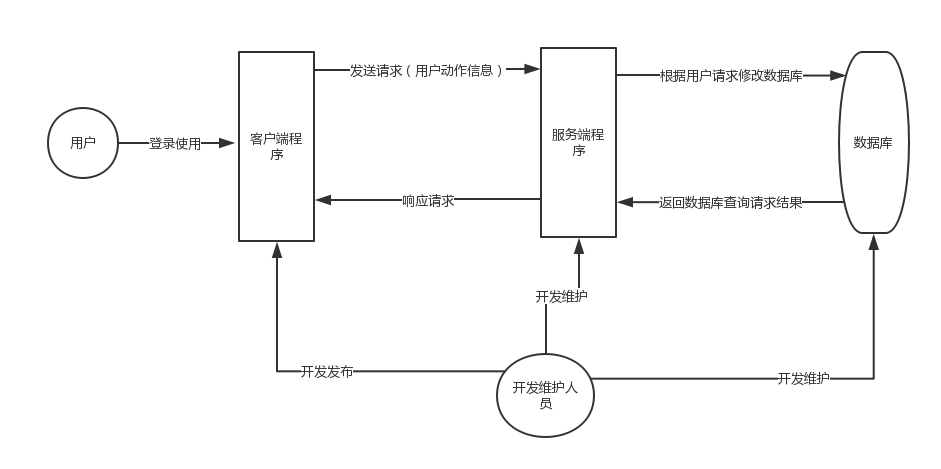
\includegraphics[width=10cm]{zhengti.png}
	\caption{系统基本流程} 
	\label{fig:figure8s}
\end{figure}

\subsection{客户端基本流程}
\begin{figure}[H]
	\centering
	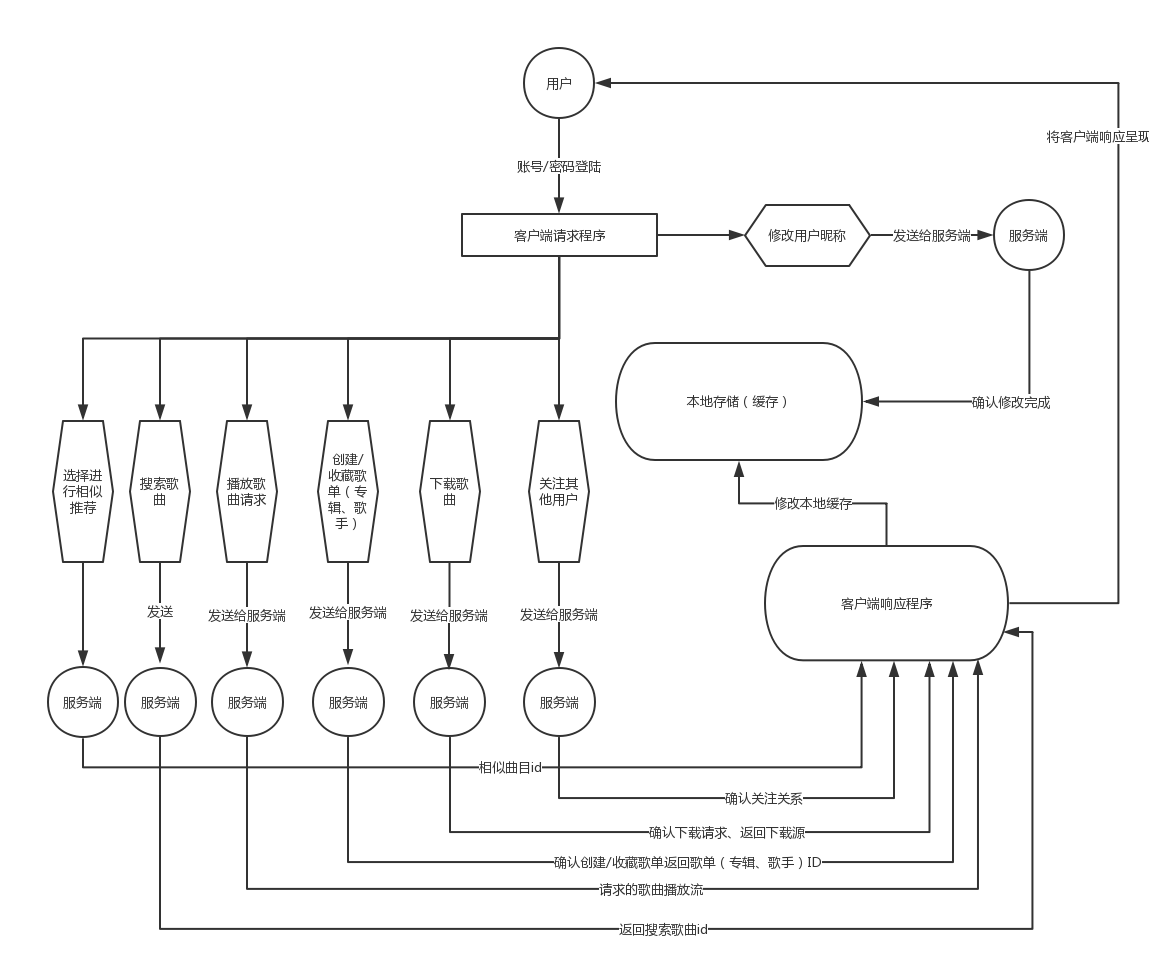
\includegraphics[width=10cm]{kehuduanchuliliucheng.png}
	\caption{客户端基本流程} 
	\label{fig:figure8d}
\end{figure}

在用户移动端上提供一个云平台的客户服务平台,主要目的在于与服务端之间建立通信关

系,产生发送对应的请求与动作,接受服务端的响应。例如接受服务端发送回来的播放的音

频流,调用播放接口对请求的歌曲进行播放,还包括例如缓存功能,缓存最近播放的歌曲在

移动端的存储中,缓存如用户昵称等个人信息。

\subsection{服务器端基本流程}

\begin{figure}[H]
	\centering
	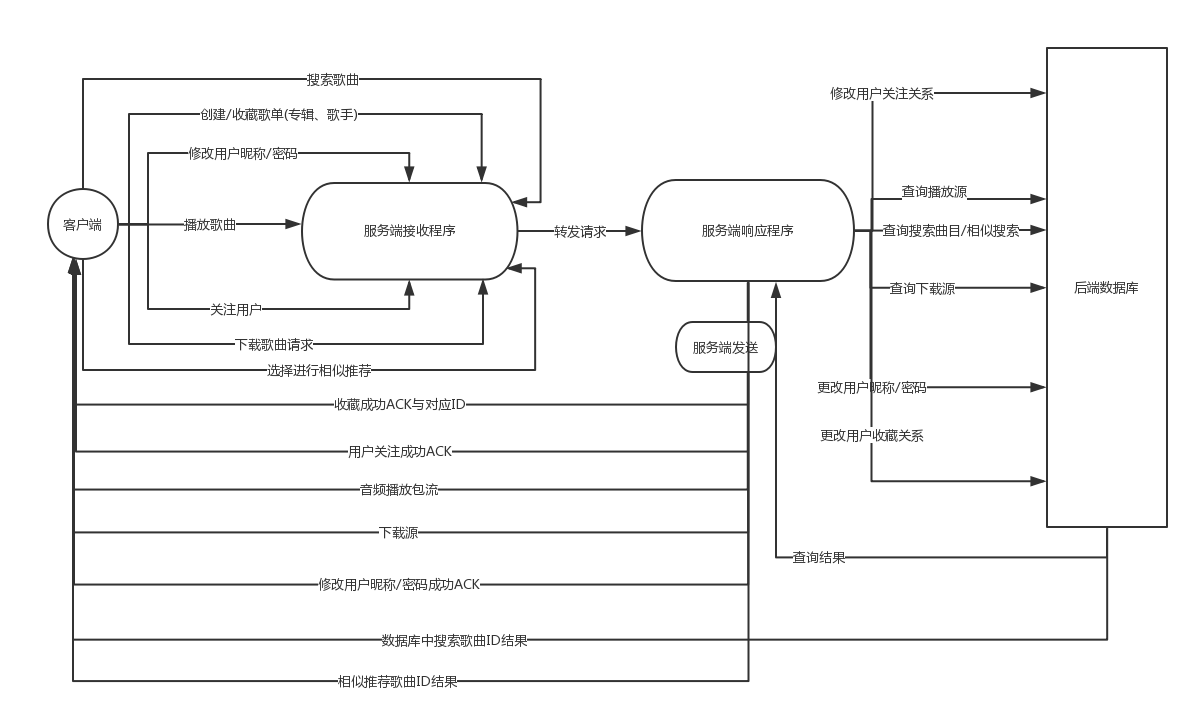
\includegraphics[width=10cm]{fuwuduanchuliliucheng.png}
	\caption{服务器端基本流程} 
	\label{fig:figure8ds}
\end{figure}
接受客户端发送的动作和请求,处理并响应,同时对该请求做出响应,例如前端某用户收藏了某歌单,客户端发送该动作,服务端做出相应的响应,将该歌单来源返回给用户,并修改相应的的数据库信息。当前端发送请求下载某歌曲,服务端响应发送歌曲下载源,对应 播放请求则就是响应发送音频包流。

\subsection{功能1搜索具体流程}

已经登录的用户在搜索栏提交get请求,客户端发送用户搜索请求数据包,提交的内容中包含歌曲的部分关键字,由服务端接收程序验证该请求是否合法,并由服务端处理程序在数据库中进行对应的查询,返回的数据包中包括包含歌曲的ID、歌曲名称、歌曲所属专辑 、歌曲演唱歌手等信息的界面。

\subsection{功能2播放具体流程}

 已经登录的用户在歌曲信息界面发送播放歌曲请求(在线缓存播放),客户端发送的数据包包括歌曲ID号等候选码,由服务端接收程序验证该请求是否合法,服务端处理程序接受请求并在数据库中进行相应搜索,将相应歌曲的音频包流发送回客户端,客户端接收程 序接收音频数据包调用本地接口对该歌曲进行播放。


\subsection{功能3收藏具体流程}


已经登录的用户在歌曲(专辑、歌手)信息界面发送收藏请求(在线缓存播放),客户端发送的数据包包括用户ID和歌曲(专辑、歌手)ID号等候选码,由服务端接收程序验证该请求是否合法,服务端处理程序接受请求并在用户信息数据库中进行相应搜索,修改数据 库中用户收藏关系条目,若成功则返回收藏成功ACK至客户端。

\subsection{功能4下载具体流程}

已经登录的用户在歌曲信息界面发送播放歌曲请求(在线缓存播放),客户端发送的数据包包括歌曲ID号等候选码,由服务端接收程序验证该请求是否合法,服务端处理程序接受请求并在数据库中进行相应搜索,将相应歌曲的下载源客户端,客户端接收程序接收下载源 ,调用本地程序接口,处理下载源请求,将下载源处的歌曲下载至本地存储。

\subsection{功能5关注用户具体流程}

已经登录的用户在其他用户界面发送播放歌曲请求(在线缓存播放),客户端发送的数据包包括发起请求用户的ID和目标用户界面的ID,由服务端接收程序验证该请求是否合法,服务端处理程序接受请求并在数据库中对发起请求用户ID进行相应搜索,将其关注用户中添 加目标用户,并搜索目标用户条目,在其粉丝成员中添加发起请求用户,完成操作后服务端发送关注成功ACK至客户端。

\subsection{功能6相似推荐具体流程}

已经登录的用户在歌曲信息界面发送相似推荐请求,客户端发送的数据包包括所在曲目歌曲ID号等候选码,由服务端接收程序验证该请求是否合法,服务端处理程序接受请求并利用推荐搜索算法在数据库中进行相应搜索,搜索相似曲风的歌曲ID及其他信息并将其发送回 客户端,客户端接收并将歌曲名称进行罗列供用户选择。

\section{功能结构设计}
\subsection{整体结构}
此处应当有一个图和对应的描述。系统如果像微内核那样,划分成核心模块和若干个子系统,此处应当有图示及说明,然后后续几个节应当描述这几个子系统。如果系统像宏内核,那应当说明有哪些紧密联系的模块,并在后续几个节内描述这些模块。
`
\subsection{客户端结构}

\begin{figure}[H]
	\centering
	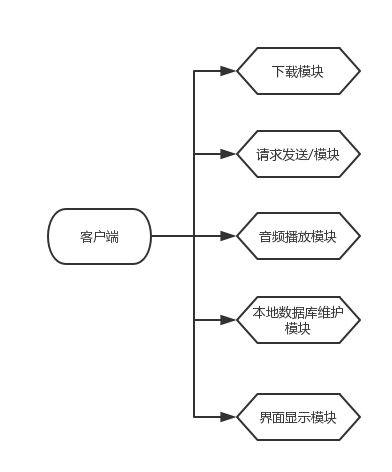
\includegraphics[width=10cm]{kehuduanjiegou.png}
	\caption{客户端结构} 
	\label{fig:figure8asd}
\end{figure}


\subsection{服务器端结构}

\begin{figure}[H]
	\centering
	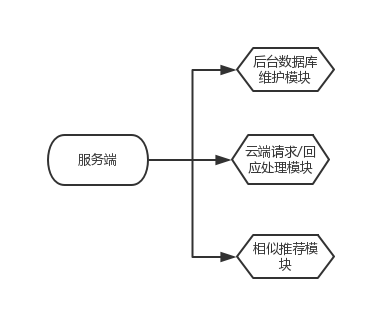
\includegraphics[width=10cm]{fuwuduanjiegou.png}
	\caption{服务器端结构} 
	\label{fig:figure8ass}
\end{figure}




\section{功能需求与程序代码的关系}
[此处指的是不同的需求分配到哪些模块去实现。可按不同的端拆分此表]
\begin{table}[htbp]
\centering
\caption{功能需求与程序代码的关系表} \label{tab:requirement-module}
\begin{tabular}{|c|c|c|c|c|c|c|c|c|c|}
    \hline
    · & 下载模块 & 请求发送/接收模块 & 音频播放模块 & 本地数据库维护模块 & 界面显示模块 & 后台数据库维护模块
     & 云端请求/回应处理模块 & 相似推荐模块 \\
    \hline
    搜索 & · & Y & . & . & .& Y& .& . \\
    \hline
    播放 & · & Y & Y & . & .& Y.& .& . \\
    \hline
    收藏 & · & Y & . & . & .& Y.& Y& . \\
    \hline
    个人信息 & · & Y & . & . & .& Y.& Y& . \\
    \hline
    推荐功能 & · & Y & . & . & .& Y.& Y& Y \\
    \hline
\end{tabular}
\note{各项功能需求的实现与各个程序模块的分配关系}
\end{table}